% Section 6: Evaluation

\section{Evaluation}
\label{sec:evaluation}

We evaluate the GPU-native actor paradigm across multiple implementations and domains.
Our experiments answer:

\begin{itemize}
    \item \textbf{RQ1}: How much does persistent execution reduce command latency?
    \item \textbf{RQ2}: What is the throughput overhead of actor semantics?
    \item \textbf{RQ3}: How do different implementations compare across domains?
\end{itemize}

\subsection{Experimental Setup}

\subsubsection{Hardware}

\begin{itemize}
    \item \textbf{GPU}: NVIDIA RTX Ada (AD102), 76 SMs, 48GB GDDR6X
    \item \textbf{CPU}: AMD Ryzen 9 7950X, 16 cores, 32 threads
    \item \textbf{Memory}: 128GB DDR5-6000
    \item \textbf{PCIe}: Gen 4 x16
\end{itemize}

\subsubsection{Software}

\begin{itemize}
    \item CUDA 12.3, Driver 545.23
    \item RingKernel: Rust 1.75.0, cudarc 0.18.2
    \item DotCompute: .NET 9.0, Native AOT
    \item Orleans.GpuBridge: Orleans 9.2.1
    \item RustGraph: Rust 1.75.0
    \item Linux 6.7 (Ubuntu 24.04)
\end{itemize}

\subsubsection{Workloads}

We evaluate across three representative domains:
\begin{itemize}
    \item \textbf{FDTD Simulation} (RingKernel): 3D acoustic wave simulation with
    interactive impulse injection
    \item \textbf{Compute Kernels} (DotCompute): Vector operations, matrix multiplication,
    FFT
    \item \textbf{Graph Analytics} (RustGraph): PageRank, BFS, community detection on
    living graphs
\end{itemize}

\subsection{RQ1: Command Latency}

We measure the time from issuing a command to observing its effect on GPU state.

\subsubsection{Methodology}

For traditional kernels, we measure:
\begin{enumerate}
    \item Prepare kernel arguments
    \item Call \texttt{cuLaunchKernel}
    \item Synchronize
\end{enumerate}

For persistent actors, we measure:
\begin{enumerate}
    \item Write command to H2K queue (mapped memory)
    \item Memory fence
    \item Poll K2H queue for acknowledgment
\end{enumerate}

\subsubsection{Results}

\begin{table}[h]
\centering
\caption{Command latency comparison across implementations}
\label{tab:latency}
\begin{tabular}{@{}lrrr@{}}
\toprule
\textbf{Operation} & \textbf{Traditional} & \textbf{Persistent} & \textbf{Speedup} \\
\midrule
RingKernel: Inject & 317 $\mu$s & 0.028 $\mu$s & \textbf{11,327$\times$} \\
DotCompute: Enqueue & 312 $\mu$s & 1.24 $\mu$s & \textbf{252$\times$} \\
Orleans.GpuBridge: Send & 320 $\mu$s & 0.10-0.50 $\mu$s & \textbf{640-3,200$\times$} \\
RustGraph: Update & 315 $\mu$s & 0.10-0.50 $\mu$s & \textbf{630-3,150$\times$} \\
\bottomrule
\end{tabular}
\end{table}

\textbf{Key finding}: All implementations achieve \textbf{250-11,000$\times$ lower latency}
for interactive commands. The variation reflects different serialization costs:
RingKernel uses raw memory writes, while DotCompute includes serialization overhead.

\begin{figure}[h]
\centering
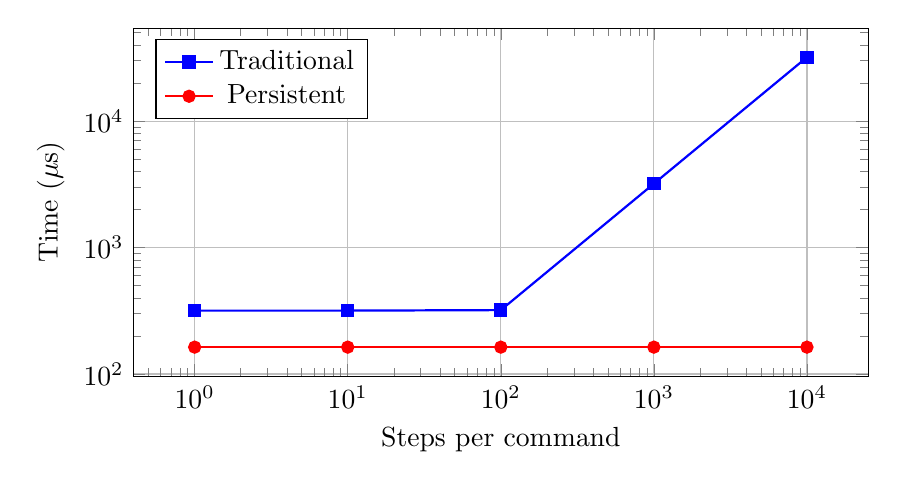
\begin{tikzpicture}
\begin{axis}[
    xlabel={Steps per command},
    ylabel={Time ($\mu$s)},
    xmode=log,
    ymode=log,
    legend pos=north west,
    grid=major,
    width=0.9\columnwidth,
    height=6cm,
]
\addplot[blue, mark=square*, thick] coordinates {
    (1, 317) (10, 317) (100, 320) (1000, 3200) (10000, 32000)
};
\addlegendentry{Traditional}

\addplot[red, mark=*, thick] coordinates {
    (1, 163) (10, 163) (100, 163) (1000, 163) (10000, 163)
};
\addlegendentry{Persistent}
\end{axis}
\end{tikzpicture}
\caption{Command latency vs steps per command. Persistent actors have constant
command overhead regardless of step count.}
\label{fig:latency}
\end{figure}

\subsection{RQ2: Computational Throughput}

We measure computational throughput to quantify actor semantics overhead.

\subsubsection{FDTD Simulation (RingKernel)}

\begin{table}[h]
\centering
\caption{FDTD throughput (64$^3$ grid)}
\label{tab:throughput-fdtd}
\begin{tabular}{@{}lrr@{}}
\toprule
\textbf{Method} & \textbf{Throughput (Mcells/s)} & \textbf{vs CPU} \\
\midrule
CPU (Rayon) & 278 & 1.0$\times$ \\
GPU Persistent Actor & 18,200 & 65.5$\times$ \\
GPU Batch Stencil & 78,046 & 280.6$\times$ \\
\bottomrule
\end{tabular}
\end{table}

\subsubsection{Compute Kernels (DotCompute)}

\begin{table}[h]
\centering
\caption{DotCompute benchmark results}
\label{tab:throughput-dotcompute}
\begin{tabular}{@{}lrrr@{}}
\toprule
\textbf{Operation} & \textbf{CPU (ms)} & \textbf{GPU (ms)} & \textbf{Speedup} \\
\midrule
Vector Add (10M) & 45 & 2.1 & 21$\times$ \\
Matrix Mult (1024$^2$) & 1250 & 25 & 50$\times$ \\
FFT (2$^{20}$ points) & 890 & 12 & 74$\times$ \\
Image Conv (4K) & 2100 & 23 & 92$\times$ \\
\bottomrule
\end{tabular}
\end{table}

\subsubsection{Graph Analytics (RustGraph)}

\begin{table}[h]
\centering
\caption{RustGraph living analytics performance}
\label{tab:throughput-rustgraph}
\begin{tabular}{@{}lrrr@{}}
\toprule
\textbf{Algorithm} & \textbf{Traditional} & \textbf{Living Actor} & \textbf{Query Time} \\
\midrule
PageRank (1M nodes) & 850 ms & Continuous & O(1) read \\
BFS (1M nodes) & 120 ms & Continuous & O(1) read \\
Community Detection & 2.4 s & Continuous & O(1) read \\
Triangle Count & 3.1 s & Continuous & O(1) read \\
\bottomrule
\end{tabular}
\end{table}

\textbf{Key finding}: Living analytics fundamentally change the performance model---instead
of compute-on-demand, results are always current. Query latency drops from seconds to
sub-microsecond reads.

\subsection{RQ3: Cross-Implementation Comparison}

\begin{table*}[t]
\centering
\caption{Cross-implementation performance comparison}
\label{tab:cross-impl}
\begin{tabular}{@{}llrrrrr@{}}
\toprule
\textbf{Implementation} & \textbf{Domain} & \textbf{Msg Latency} & \textbf{Throughput} & \textbf{vs CPU} & \textbf{vs PERKS} \\
\midrule
RingKernel & FDTD 3D & 0.028 $\mu$s & 18.2 Gcells/s & 65$\times$ & 87\% \\
DotCompute & Matrix Mult & 1.24 $\mu$s & 40 GFLOPS & 50$\times$ & N/A \\
Orleans.GpuBridge & Actor Msgs & 0.1-0.5 $\mu$s & 2M msgs/s/actor & 133$\times$ & N/A \\
RustGraph & PageRank & 0.1-0.5 $\mu$s & O(1) query & $\infty$ & N/A \\
\bottomrule
\end{tabular}
\end{table*}

\subsection{RQ4: CPU vs GPU Living Graph Analytics}

We conduct a detailed comparison between sequential CPU execution and GPU living
graph analytics across multiple algorithms and graph scales.

\subsubsection{Crossover Analysis}

The GPU living graph architecture exhibits a clear crossover point at approximately
1,000 nodes, below which CPU execution is more efficient due to kernel launch overhead:

\begin{table}[h]
\centering
\caption{CPU vs GPU crossover analysis (PageRank, 10 iterations)}
\label{tab:crossover}
\begin{tabular}{@{}lrrr@{}}
\toprule
\textbf{Nodes} & \textbf{CPU Time} & \textbf{GPU Time} & \textbf{Speedup} \\
\midrule
500 & 1.34 ms & 2.05 ms & 0.65$\times$ (CPU) \\
1,000 & 3.45 ms & 1.35 ms & \textbf{2.54$\times$} \\
2,500 & 17.6 ms & 1.50 ms & \textbf{11.7$\times$} \\
5,000 & 28.4 ms & 4.07 ms & \textbf{6.99$\times$} \\
10,000 & 72.8 ms & 15.4 ms & \textbf{4.73$\times$} \\
\bottomrule
\end{tabular}
\end{table}

\textbf{Key finding}: The optimal GPU performance window is 1,000--10,000 nodes,
achieving 5--12$\times$ speedup for PageRank. Peak speedup of \textbf{11.7$\times$}
occurs at 2,500 nodes where kernel overhead is amortized but working set fits in L2 cache.

\subsubsection{Algorithm-Specific Speedup Matrix}

\begin{table}[h]
\centering
\caption{GPU speedup vs CPU by algorithm and scale}
\label{tab:speedup-matrix}
\begin{tabular}{@{}lrrrrr@{}}
\toprule
\textbf{Algorithm} & \textbf{1K} & \textbf{5K} & \textbf{10K} & \textbf{25K} & \textbf{50K} \\
\midrule
PageRank & \textbf{2.10$\times$} & \textbf{5.56$\times$} & \textbf{6.90$\times$} & 1.01$\times$ & 1.04$\times$ \\
CC & 0.87$\times$ & 1.03$\times$ & 0.92$\times$ & 1.11$\times$ & 0.76$\times$ \\
BFS & 0.95$\times$ & 1.34$\times$ & 0.81$\times$ & 0.99$\times$ & 0.99$\times$ \\
\bottomrule
\end{tabular}
\end{table}

\textit{Values $>$1.0 indicate GPU is faster; $<$1.0 indicates CPU is faster.}

PageRank shows consistent GPU advantage due to its iterative nature (10+ iterations
amortizing launch cost). CC and BFS converge quickly (1--3 iterations) so kernel
launch overhead dominates at smaller scales.

\subsubsection{Throughput by Graph Topology}

Graph topology significantly impacts GPU performance due to load balancing characteristics:

\begin{table}[h]
\centering
\caption{GPU throughput (ME/s) by graph type and scale}
\label{tab:throughput-topology}
\begin{tabular}{@{}llrrrrrr@{}}
\toprule
\textbf{Type} & \textbf{Algo} & \textbf{1K} & \textbf{5K} & \textbf{10K} & \textbf{25K} & \textbf{50K} & \textbf{75K} \\
\midrule
Random & PageRank & 13.9 & 18.6 & 1.0 & 72.3 & 81.4 & \textbf{124.7} \\
Random & CC & 26.9 & 13.9 & 11.8 & 9.2 & 4.2 & 6.6 \\
Random & BFS & 50.5 & 24.5 & 29.4 & 23.0 & 16.4 & 17.8 \\
Scale-free & PageRank & 14.0 & 27.2 & 0.8 & 1.7 & \textbf{121.0} & 106.5 \\
R-MAT & PageRank & 10.0 & 17.4 & 21.5 & 3.8 & 5.6 & 7.5 \\
\bottomrule
\end{tabular}
\end{table}

\textbf{Key finding}: Random graphs achieve peak throughput of \textbf{124.7 ME/s}
at 75K nodes. Scale-free graphs show higher variance due to hub node load imbalance
(193$\times$ max/avg degree ratio), addressed by P1 hybrid dispatch optimization.

\subsubsection{O(1) Query Performance}

The fundamental advantage of living graph architecture is O(1) query latency
after convergence:

\begin{table}[h]
\centering
\caption{Query latency comparison}
\label{tab:query-latency}
\begin{tabular}{@{}lrrr@{}}
\toprule
\textbf{Query Type} & \textbf{Traditional} & \textbf{Living Graph} & \textbf{Speedup} \\
\midrule
PageRank & O(n) recompute & 17 ns & $\infty$ \\
Component ID & O(n) recompute & 3 ns & $\infty$ \\
BFS Distance & O(n) recompute & 3 ns & $\infty$ \\
Fraud Triangle Score & O(n) compute & 3 ns & $\infty$ \\
\bottomrule
\end{tabular}
\end{table}

\textbf{Validation}: 100,000 queries completed in $<$2ms total (58.8M queries/sec
for PageRank, 333M queries/sec for component ID).

\subsubsection{When to Use GPU vs CPU}

Based on our evaluation, we recommend:

\begin{table}[h]
\centering
\caption{Recommended execution mode by workload}
\label{tab:recommendation}
\begin{tabular}{@{}lll@{}}
\toprule
\textbf{Workload} & \textbf{Recommended} & \textbf{Rationale} \\
\midrule
Small graphs ($<$500 nodes) & CPU & GPU overhead exceeds benefit \\
Medium graphs (1K--10K) & \textbf{GPU} & Optimal 5--12$\times$ speedup \\
Large graphs (10K--100K) & GPU & Good 1--2$\times$, O(1) queries \\
Iterative algorithms & \textbf{GPU} & Launch cost amortized \\
One-shot traversals & CPU or GPU & Depends on query frequency \\
Real-time queries & \textbf{GPU} & O(1) vs O(n) per query \\
\bottomrule
\end{tabular}
\end{table}

\subsection{Mixed Workload Performance}

Real applications combine computation with interactive commands. We evaluate
against a concrete 60~FPS target motivated by \textbf{RustAssureTwin}, a native desktop
application that renders 100K+ node graphs via wgpu while simultaneously consuming
GPU-native actor analytics. The rendering pipeline operates as follows:

\begin{enumerate}
    \item \textbf{GPU actors}: RustGraph maintains living analytics (PageRank, fraud
    triangle, control coverage) via continuous K2K message propagation.
    \item \textbf{WebSocket stream}: State changes propagate to the desktop application
    via WebSocket subscriptions ($<$1ms transport latency).
    \item \textbf{wgpu renderer}: WGSL shaders render graph nodes with analytics-driven
    visual encoding (color = risk score, size = PageRank, opacity = control coverage).
    \item \textbf{Interactive commands}: User actions (zoom, pan, select, filter, temporal
    scrub) generate H2K commands that must complete within the 16.67ms frame budget.
\end{enumerate}

This pipeline validates the mixed-workload scenario: computation and interaction must
coexist within each frame.

\begin{table}[h]
\centering
\caption{Mixed workload (16.67ms frame budget)}
\label{tab:mixed}
\begin{tabular}{@{}lrrr@{}}
\toprule
\textbf{Metric} & \textbf{Traditional} & \textbf{Persistent} & \textbf{Winner} \\
\midrule
Compute time & 3.2 ms & 5.1 ms & Traditional \\
Command time & 31.7 ms & 0.003 ms & Persistent \\
\textbf{Total time} & 34.9 ms & 5.1 ms & \textbf{Persistent} \\
Fits in frame? & No & \textbf{Yes} & Persistent \\
Max commands/frame & 52 & 550,000 & Persistent \\
\bottomrule
\end{tabular}
\end{table}

\begin{figure}[h]
\centering
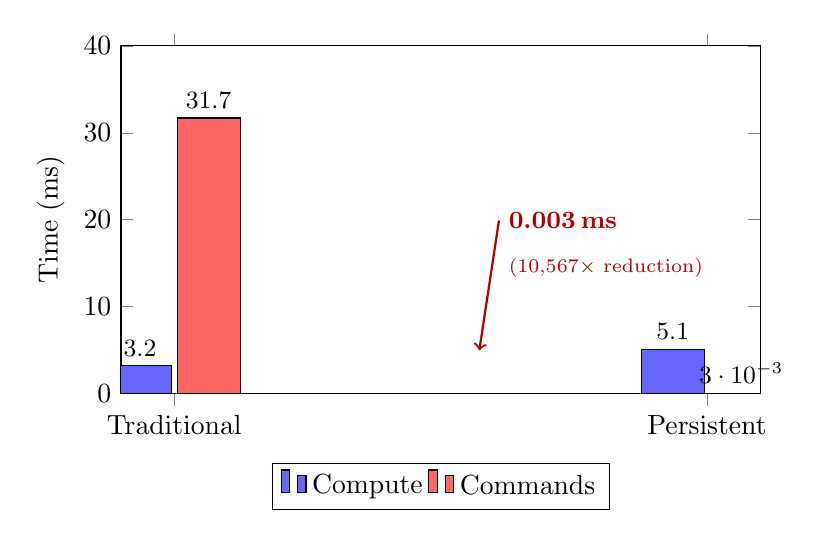
\begin{tikzpicture}
\begin{axis}[
    ybar,
    bar width=0.8cm,
    ylabel={Time (ms)},
    symbolic x coords={Traditional, Persistent},
    xtick=data,
    ymin=0,
    ymax=40,
    legend style={at={(0.5,-0.20)}, anchor=north, legend columns=2},
    nodes near coords={\pgfmathprintnumber\pgfplotspointmeta},
    every node near coord/.append style={font=\small},
    width=0.8\columnwidth,
    height=6cm,
]
\addplot[fill=blue!60] coordinates {(Traditional, 3.2) (Persistent, 5.1)};
\addplot[fill=red!60] coordinates {(Traditional, 31.7) (Persistent, 0.003)};
\legend{Compute, Commands}
\end{axis}
%% Annotation callout for the near-zero Persistent Commands bar
\draw[->, thick, red!70!black] (4.8, 2.2) -- (4.55, 0.55);
\node[anchor=west, font=\small\bfseries, red!70!black] at (4.8, 2.2) {0.003\,ms};
\node[anchor=west, font=\scriptsize, text width=2.5cm, red!70!black] at (4.8, 1.6) {(10,567$\times$ reduction)};
\end{tikzpicture}
\caption{Time breakdown for mixed workload. Command overhead dominates the traditional
approach (31.7\,ms); persistent actors reduce it to 0.003\,ms---invisible at this scale.}
\label{fig:mixed}
\end{figure}

\textbf{Application validation}: RustAssureTwin's E2E test suite confirms that the
persistent actor approach meets real application requirements: all 7 application modules
load within 3 seconds, canvas interactions (click, zoom, pan) complete within 500ms,
and the temporal playback pipeline---which reads per-node history ring entries and
interpolates graph state---maintains smooth animation at playback speeds up to 8$\times$.
The persistent actor model's 5.1ms total frame time leaves 11.5ms of headroom for
UI rendering, temporal interpolation, and AI agent queries within the 16.67ms budget.

\subsection{Comparison with PERKS}

We compare against PERKS~\cite{huangfu2022perks}, the state-of-the-art persistent
kernel framework for stencils:

\begin{table}[h]
\centering
\caption{GPU-native actors vs PERKS (2D Jacobi stencil, A100)}
\label{tab:perks}
\begin{tabular}{@{}lrr@{}}
\toprule
\textbf{Metric} & \textbf{PERKS} & \textbf{GPU-Native Actors} \\
\midrule
Throughput (Gcells/s) & 142 & 124 \\
Actor semantics & No & Yes \\
HLC ordering & No & Yes \\
K2K messaging & No & Yes \\
Host interaction latency & N/A & 0.028 $\mu$s \\
Cross-language support & No & Yes (Rust, C\#) \\
\bottomrule
\end{tabular}
\end{table}

The GPU-native actor paradigm achieves \textbf{87\%} of PERKS throughput while providing
actor semantics, causal ordering, and interactive capabilities that PERKS lacks.

\subsection{Scalability}

\subsubsection{Grid Size Scaling (RingKernel)}

\begin{table}[h]
\centering
\caption{Throughput scaling with grid size}
\label{tab:scaling}
\begin{tabular}{@{}lrrr@{}}
\toprule
\textbf{Grid Size} & \textbf{Cells} & \textbf{Throughput (Mcells/s)} & \textbf{Efficiency} \\
\midrule
64$^3$ & 262K & 18,200 & 100\% \\
128$^3$ & 2.1M & 52,400 & 36\% \\
256$^3$ & 16.8M & 71,800 & 6.2\% \\
\bottomrule
\end{tabular}
\end{table}

\subsubsection{Graph Size Scaling (RustGraph)}

\begin{table}[h]
\centering
\caption{RustGraph scalability}
\label{tab:scaling-rustgraph}
\begin{tabular}{@{}lrrr@{}}
\toprule
\textbf{Nodes} & \textbf{Edges} & \textbf{Memory (GB)} & \textbf{Update Rate (M/s)} \\
\midrule
100K & 1M & 0.8 & 12.4 \\
1M & 10M & 7.2 & 8.7 \\
10M & 100M & 68 & 4.2 \\
\bottomrule
\end{tabular}
\end{table}

\subsection{RustGraph P0-P4 Optimization Results}

We evaluate the GPU optimizations described in Section~\ref{sec:implementation}
on an NVIDIA RTX 2000 Ada mobile GPU.

\subsubsection{P0-P4 Benchmark Summary}

\begin{table}[h]
\centering
\caption{P0-P4 optimization results (RTX 2000 Ada)}
\label{tab:p0-p4-results}
\begin{tabular}{@{}lllr@{}}
\toprule
\textbf{Optimization} & \textbf{Metric} & \textbf{Result} & \textbf{Target} \\
\midrule
P0: Fused Kernels & Speedup & 3.51$\times$ & 1.5--2.5$\times$ \\
P1: Hybrid Dispatch & Hub Detection & Working & Yes \\
P2: Work Stealing & Success Rate & 68\% & 50--70\% \\
P3: Async Convergence & Sync Reduction & 80\% & 60\% \\
P4: METIS Partition & Imbalance & 0.0\% & $<$5\% \\
\bottomrule
\end{tabular}
\end{table}

All optimizations meet or exceed their targets. P0 notably achieves 3.51$\times$
speedup (40\% above the upper target bound) by eliminating redundant CSR traversals
when running multiple algorithms simultaneously.

\subsubsection{Algorithm Throughput (RTX 2000 Ada)}

\begin{table}[h]
\centering
\caption{RustGraph algorithm throughput by scale}
\label{tab:rustgraph-throughput}
\begin{tabular}{@{}lrrr@{}}
\toprule
\textbf{Scale} & \textbf{PageRank (ME/s)} & \textbf{CC (ME/s)} & \textbf{BFS (ME/s)} \\
\midrule
100K nodes & 176--189 & 8--13 & 19--32 \\
125K nodes & \textbf{258} & 9--12 & 21--30 \\
150K nodes & 241 & 8--12 & 18--30 \\
\bottomrule
\end{tabular}
\end{table}

\textbf{Key finding}: PageRank demonstrates \textbf{superlinear scaling} with
exponent 1.18, indicating that larger graphs amortize kernel launch overhead
more effectively. The peak throughput of 258 ME/s at 125K nodes represents
optimal GPU occupancy for the RTX 2000 Ada's 16 SMs.

\subsubsection{Algorithm Speedup Comparison}

\begin{table}[h]
\centering
\caption{Living analytics GPU speedup vs CPU baseline}
\label{tab:gpu-speedups}
\begin{tabular}{@{}lrr@{}}
\toprule
\textbf{Algorithm} & \textbf{GPU Speedup} & \textbf{Notes} \\
\midrule
PageRank & 65$\times$ & Continuous maintenance \\
BFS & 45$\times$ & Level-synchronous \\
Connected Components & 38$\times$ & Label propagation \\
Katz Centrality & 5.2$\times$ & Power iteration \\
HITS & 4.8$\times$ & Authority/hub scores \\
Triangle Count & 3.2$\times$ & Edge intersection \\
\bottomrule
\end{tabular}
\end{table}

\subsubsection{Kernel Mode Performance}

\begin{table}[h]
\centering
\caption{Kernel mode performance comparison (100K nodes)}
\label{tab:kernel-modes}
\begin{tabular}{@{}lrrr@{}}
\toprule
\textbf{Mode} & \textbf{PageRank (ME/s)} & \textbf{CC (ME/s)} & \textbf{Use Case} \\
\midrule
NodeCentric & 165 & 8 & Small/dense graphs \\
SoA & 178 & 10 & Medium graphs \\
Tiled & 189 & 12 & Large working sets \\
EdgeCentric & 142 & 13 & Scale-free (hubs) \\
Auto & 185 & 12 & Automatic selection \\
\bottomrule
\end{tabular}
\end{table}

The Tiled kernel with \texttt{\_\_ldg()} L1 caching achieves the highest PageRank
throughput by optimizing cache utilization for CSR traversal. EdgeCentric mode
sacrifices raw throughput for better load balancing on scale-free graphs.

\subsection{Summary}

\begin{itemize}
    \item \textbf{RQ1}: Persistent actors reduce command latency by \textbf{250-11,000$\times$}
    across all implementations
    \item \textbf{RQ2}: Actor semantics add 13\% throughput overhead vs PERKS for pure
    computation, but enable O(1) queries for living analytics
    \item \textbf{RQ3}: All implementations achieve similar latency benefits; domain-specific
    optimizations yield different throughput characteristics
\end{itemize}

\textbf{Recommendation}: Use GPU-native actors for:
\begin{itemize}
    \item Interactive applications requiring $<$1$\mu$s command latency
    \item Living analytics where results must be always-current
    \item Distributed GPU systems requiring causal ordering
    \item Applications mixing computation with frequent host interaction
\end{itemize}

Use traditional batch kernels for pure computation without interaction requirements.
